
\noindent\begin{minipage}{\textwidth}
    \begin{table}[H]
        \centering
        \caption{Hiperparâmetros e Resultados do Melhor Modelo - vgg\_v12\_BR\_opt\_aug}
        \vspace{0.2cm}
        \resizebox{\textwidth}{!}{%
            \begin{tabular}{ll | lrrr}
                \hline
                \multicolumn{2}{c|}{\textbf{Hiperparâmetros}} & \multicolumn{4}{c}{\textbf{Métricas por Classe}} \\ \hline
                \textbf{Parâmetro} & \textbf{Valor} & \textbf{Classe} & \textbf{Precisão} & \textbf{Recall} & \textbf{F1-Score} \\ \hline
    Agendador (Patience) & 6 & 31.2 & 0,4386 & 0,5631 & 0,4931 \\ 
Agendador de LR & ReduceLROnPlateau & 31.3 & 0,2333 & 0,3723 & 0,2869 \\ 
Architecture & vgg19\_bn & 31.4 & 0,3450 & 0,2588 & 0,2957 \\ 
Augmentation (Método) & None & 32.3 & 0,4554 & 0,2434 & 0,3172 \\ 
Batch Size & 32 & 32.4 & 0,4545 & 0,1389 & 0,2128 \\ 
Decaimento de Peso (WD) & 0,0008 & 33.3 & 0,3060 & 0,4491 & 0,3640 \\ 
Dropout & 0,6374 & 41.4 & 0,1935 & 0,1277 & 0,1538 \\ 
Função de Perda & CrossEntropyLoss & 41.5 & 0,5333 & 0,3721 & 0,4384 \\ 
Hidden Units & 256 & 42.4 & 0,2500 & 0,0164 & 0,0308 \\ 
Label Smoothing & 0,0000 & 44.4 & 0,2500 & 0,0938 & 0,1364 \\ 
\cline{3-6} 
Otimizador & SGD & \textbf{Média (Macro)} & 0,3460 & 0,2635 & 0,2729 \\ 
Taxa de Aprendizado (LR) & 6,68e-03 & \textbf{MCC} & \multicolumn{3}{c}{0,2197} \\ 
Unfreeze Layers & 5 &  & & &  \\ 
            \hline
            \end{tabular}%
        }
    \end{table}

    \begin{figure}[H]
        \centering
        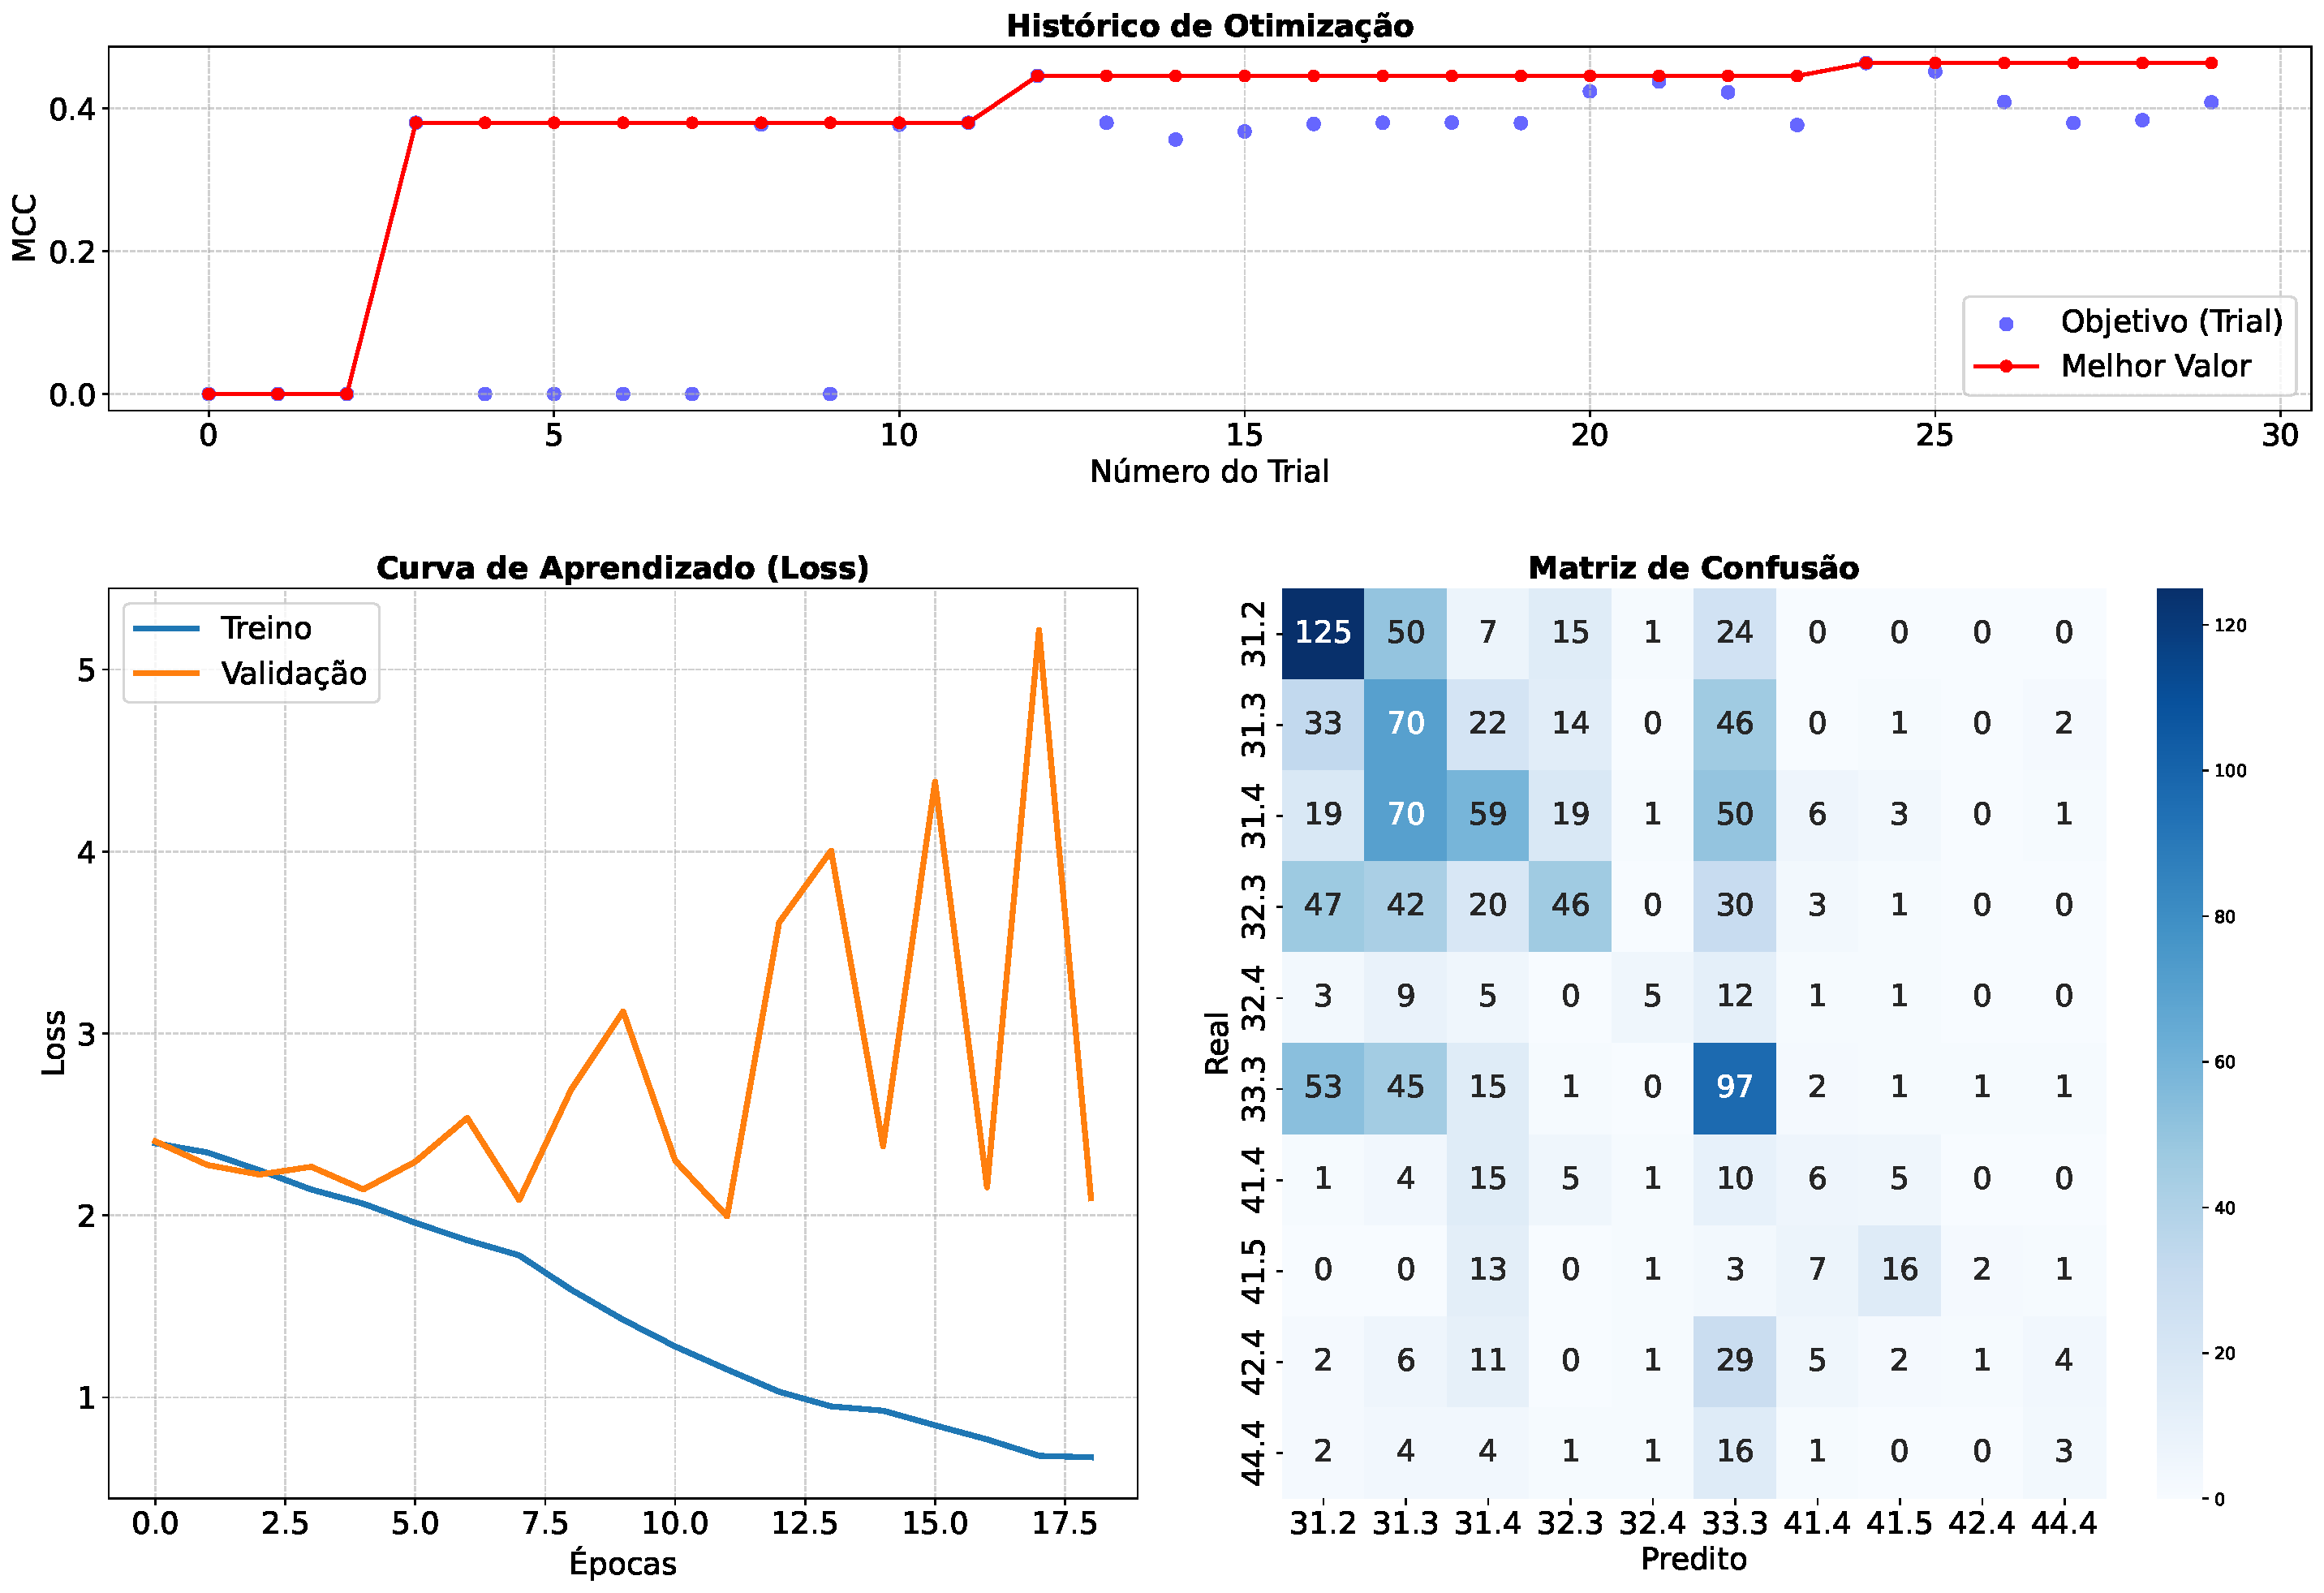
\includegraphics[width=0.85\textwidth]{tex/appendix/experiments/vgg_v12_BR_opt_aug/dashboard_consolidado.pdf}
        \caption{Histórico de Otimização, Curvas de Aprendizado e Matriz de Confusão - vgg\_v12\_BR\_opt\_aug}
    \end{figure}
\end{minipage}
\clearpage
